\section{Analyses \& Results}
\label{sec_analyses}

\subsection{RQ1: Comparison of tagged and untagged time series}
Our principal research question is whether listening patterns for tagged content are consistent with the expectation that tags serve as memory cues. If this were to be the case, we would expect to see increased listening rates for musical artists once a tag is applied, under the assumption that a tag facilitates retrieval and increases the chances of a user listening to a tagged artist. 

Unfortunately, several factors combine to make such an analysis difficult.  First and foremost, the desired counterfactual of the untagged ``version'' of a particular tagged series, which would allow a direct testing of how tagging changes listening behavior, does not, of course, exist. We thus must utilize untagged time series in a way that allows them to approximate what a true counterfactual might look like.  In searching for such samples, a second difficulty that arises is that listening rates for tagged time series are much greater than for untagged time series (the average number of total listens across time series is 16.9 when untagged and 98.9 when tagged). While suggestive of the importance of tagging, this unbalance also suggests that controls must be instilled in both sample selection and statistical analysis to account for previous listening behavior prior to tagging. Finally, the actual point in time at which tags are expected to increase listening behavior for any given user is unknown, as it is theoretically possible that tagging may affect listening behavior as much three months after the tag has been placed as it does in the immediately following month.  Thus, we must formulate our analysis in such a fashion as to account for this possibility.  
%to understand how it changes behavior

%meticulously
To alleviate issues with the non-existence of a true counterfactual, we subselect from both the tagged and untagged series using the following formal procedure. We first temporally align the tagged and untagged time series. Both tagged time series are aligned so that they are centered on the month in which they were tagged.  If multiple tags were present, we selected the tag within the month which had the most corresponding scrobbles. While there is no analogue to this point in the untagged data, we can partially resolve the issue by noting that tagging is disproportionately likely (approximately 30\%, compared to 1.1\% if the tagging month were random) to occur in a user's \emph{peak}\footnote{The month in which they listen the most times overall} listening month for a given artist. This provides a basis for aligning the tagged and untagged time series, by selecting only those tagged time series where the tag was applied in the month of peak listening, and then collecting a sample of untagged time series also aligned at the peak of listening.  Where the peak was reached in multiple months, we chose one of these at random.

After aligning all tagged and untagged samples in this fashion, we further limited our analysis to a 13 month period extending from 6 months prior to the peak month to 6 months after the peak. This allows us to consider a variety of ways in which listening prior to the tag may affect future behavior while still admitting that there is likely a reasonable span in which tagging and past listening behavior have an effect on future actions. Finally, we further constrain our sampling to time series with:
\begin{itemize}
\item more than 25 total listens; 
\item a peak in listening at least 6 months from the edges of our data collection period (i.e. ensuring that the period from 6 months before to 6 months after the peak does not extend beyond the limits of our data range); and
\item at least one listen 6 months prior to and after the peak (i.e. if the peak occurs in July, there should be at least one listen between January and June, and one between August and the following January).
\end{itemize}

Constraining our time series in this manner, we are left with a total of 206,140 tagged time series.  We then randomly sampled from the 4.1M untagged time series an equal number meeting the same three criteria.  All results below have been verified with multiple random samplings of the untagged data.

In Figure~\ref{fig:taggedVsUntagged} we plot mean playcounts, with 95\% normal confidence intervals, for each month across all tagged and untagged time series in the subsampled data. All values are normalized by the peak, and thus values at the peak month for both the tagged and untagged lines are unity. By visually comparing the line heights before and after the peak, Figure~\ref{fig:taggedVsUntagged} shows that the mean normalized listening rate increases in the months after the peak for both tagged and untagged time series. However, we also see a small but reliable effect wherein tagged time series show proportionally higher mean normalized listening rates after the peak month (in which the the tag was applied) as compared to untagged time series. This is suggestive of an increase in listening as a result of tagging.

While Figure~\ref{fig:taggedVsUntagged} thus gives evidence that supports our hypothesis, there are two important caveats to the data in the plot. First, because listening distributions are heavily skewed for any given month, the mean is not necessarily representative of the data. Though qualitative plots of transformed variables proved to be similar, further statistical analysis uses a log transformed version of the listening counts to account for these deviations. Second, while normalization controls for differences in listening counts between tagged and untagged data to some extent, we would prefer a method that explicitly accounts for listening behavior prior to and including the peak month on future behavior.

To more robustly test our hypothesis, we thus utilize a regression model relating post- and pre-peak listening behavior. Due to the volume of data we are dealing with, it was unreasonable make the assumption of linear dependence of the dependent variable on the independent variables. We therefore opted for a Generalized Additive Model (GAM, \cite{hastie1990generalized}), for which we utilized the R package mgcv \cite{wood2001mgcv}.
Our dependent variable in the regression is the logarithm of the sum of all listens in the six months after a tag has been applied, as we are unsure at what point post-tagging the effect of a tag may be relevant.\footnote{Qualitatively, our results hold when testing listening for each individual month as well. Also of note is our choice of using the log of the dependent variable rather than a count-based regression model (e.g. a Negative Binomial regression). The model used here appeared to fit the data better based on a variety of statistical and visual goodness-of-fit tests.} Our independent variables are an indicator of whether or not the time series has been tagged, as well seven continuous-valued predictors, one each for the logarithm of the sum of listens in the peak month and the six previous months.   

  \begin{figure}
    \subfloat[Mean normalized playcount by month. \label{fig:taggedVsUntagged}]{%
      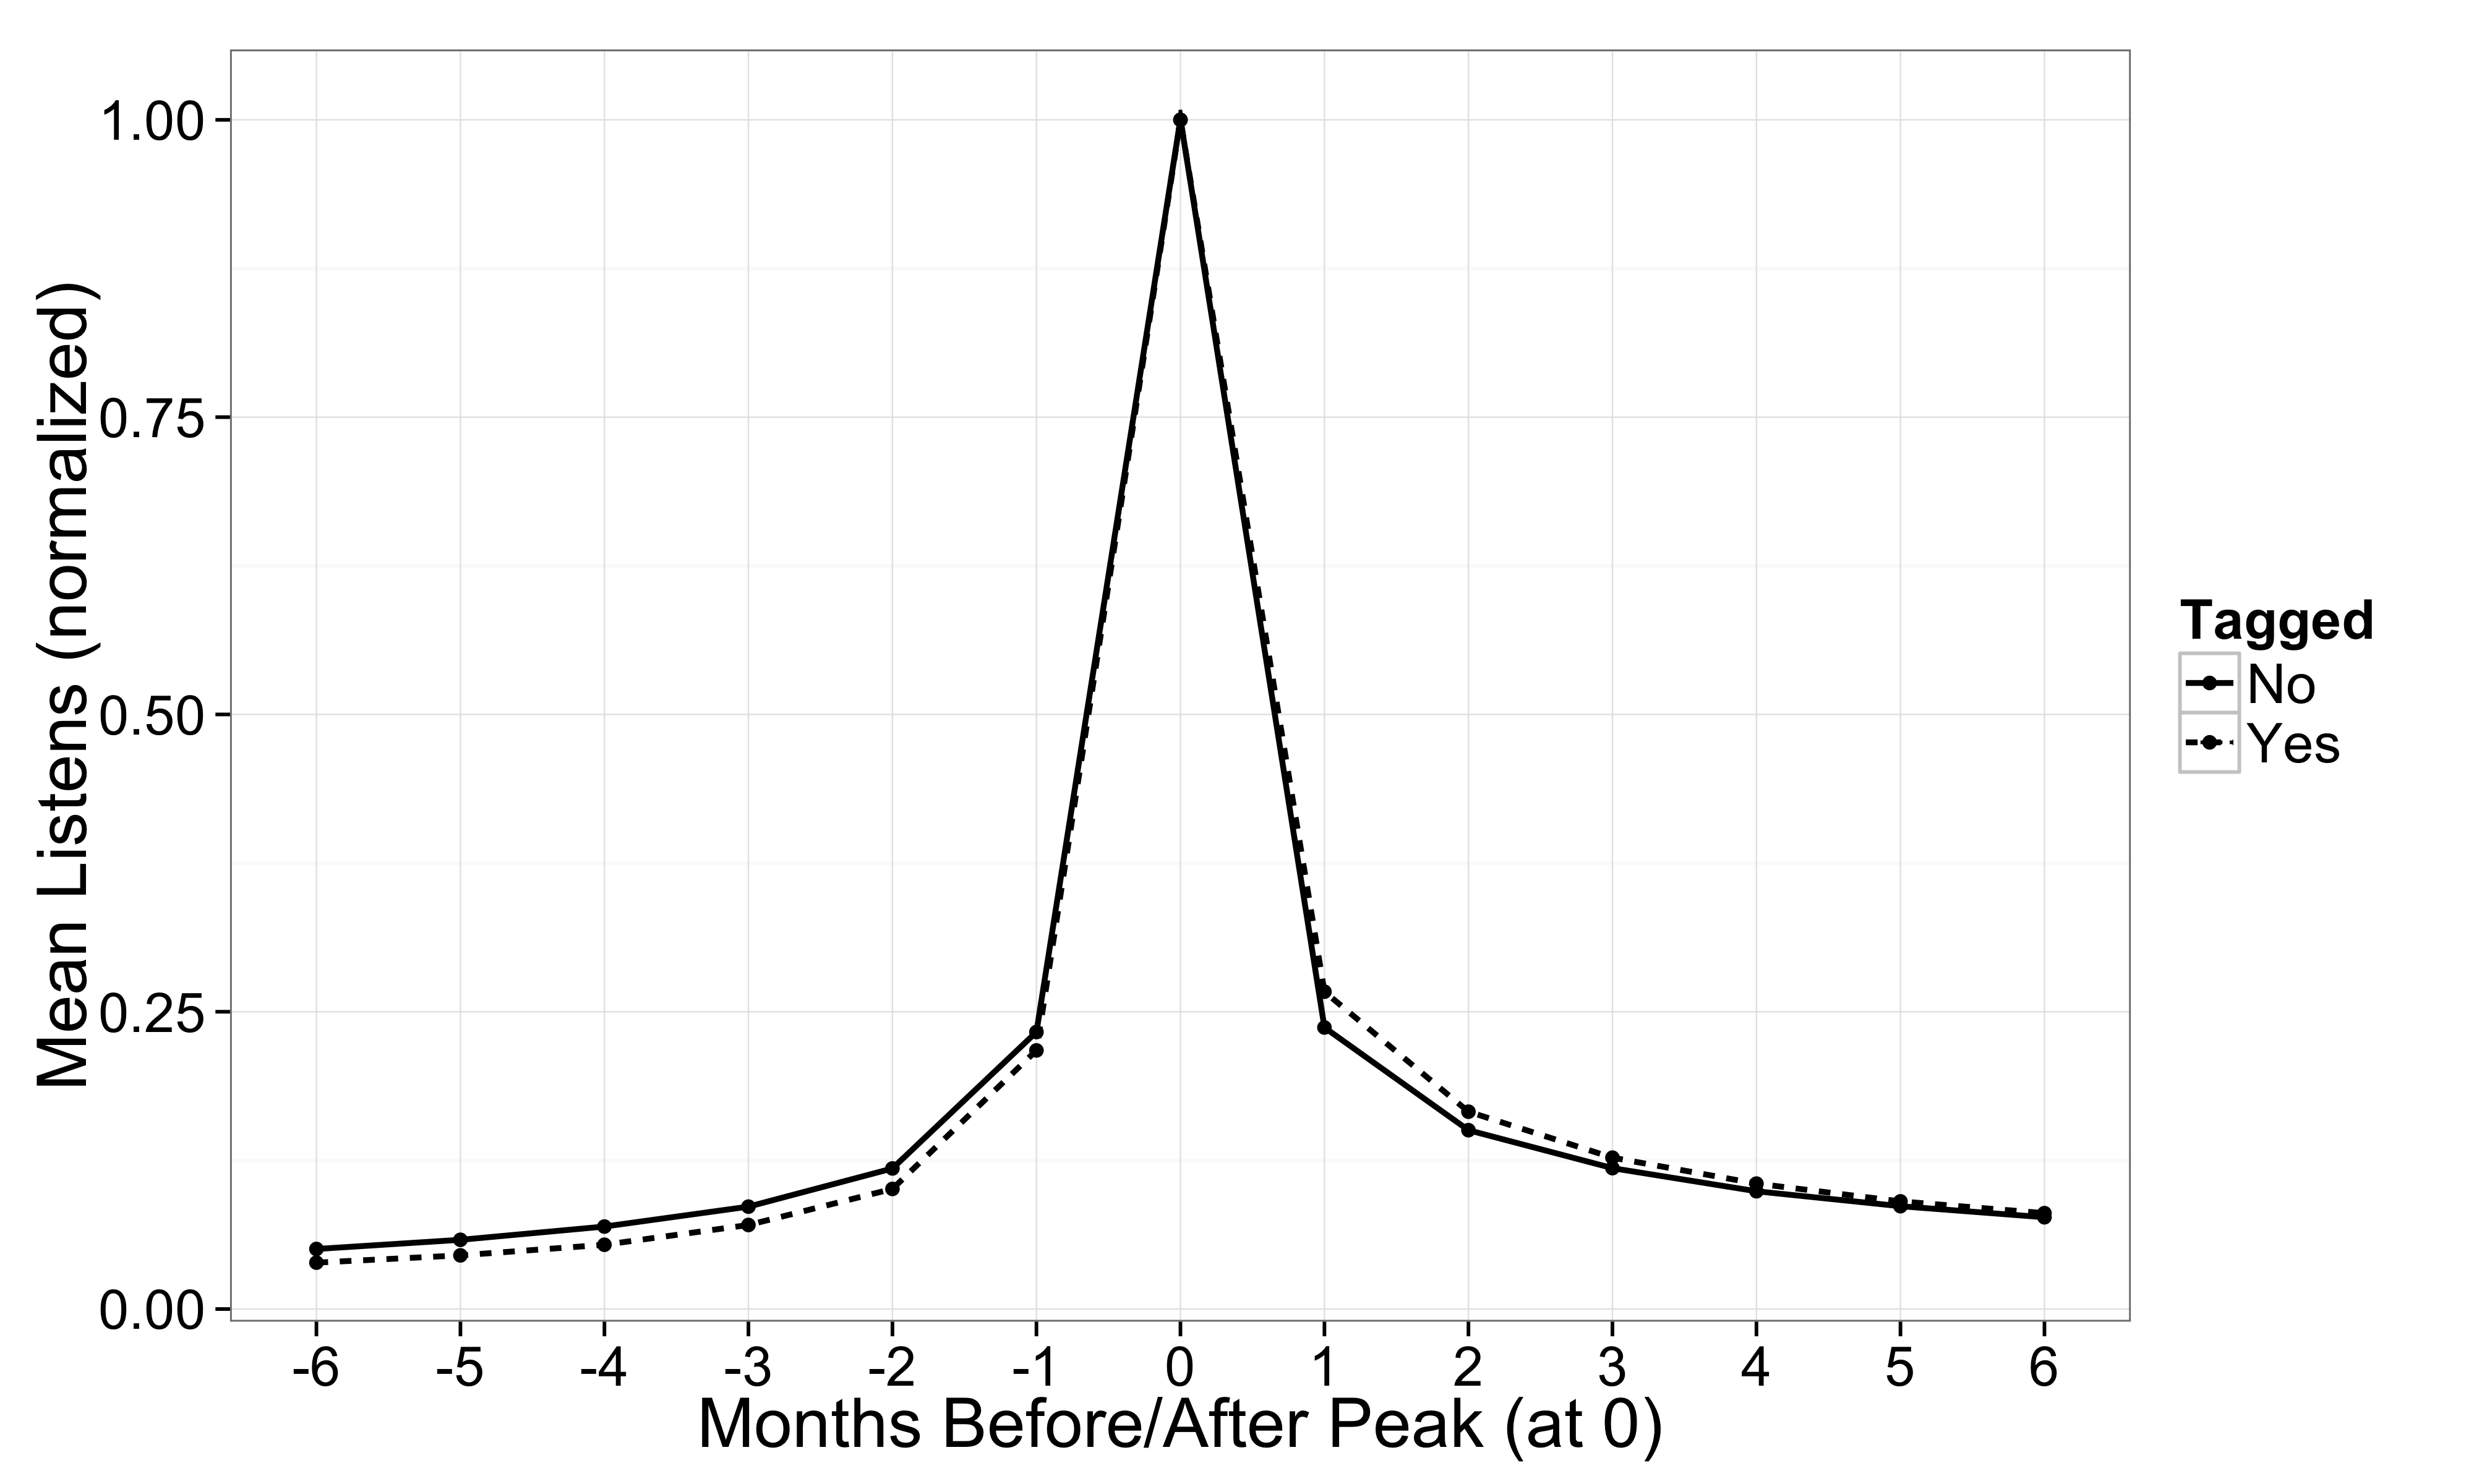
\includegraphics[width=0.5\textwidth]{taggedVUntaggedSimple.png}
    }
    \hfill
    \subfloat[Regression results, with 95\% confidence interval. \label{fig:regression}]{%
      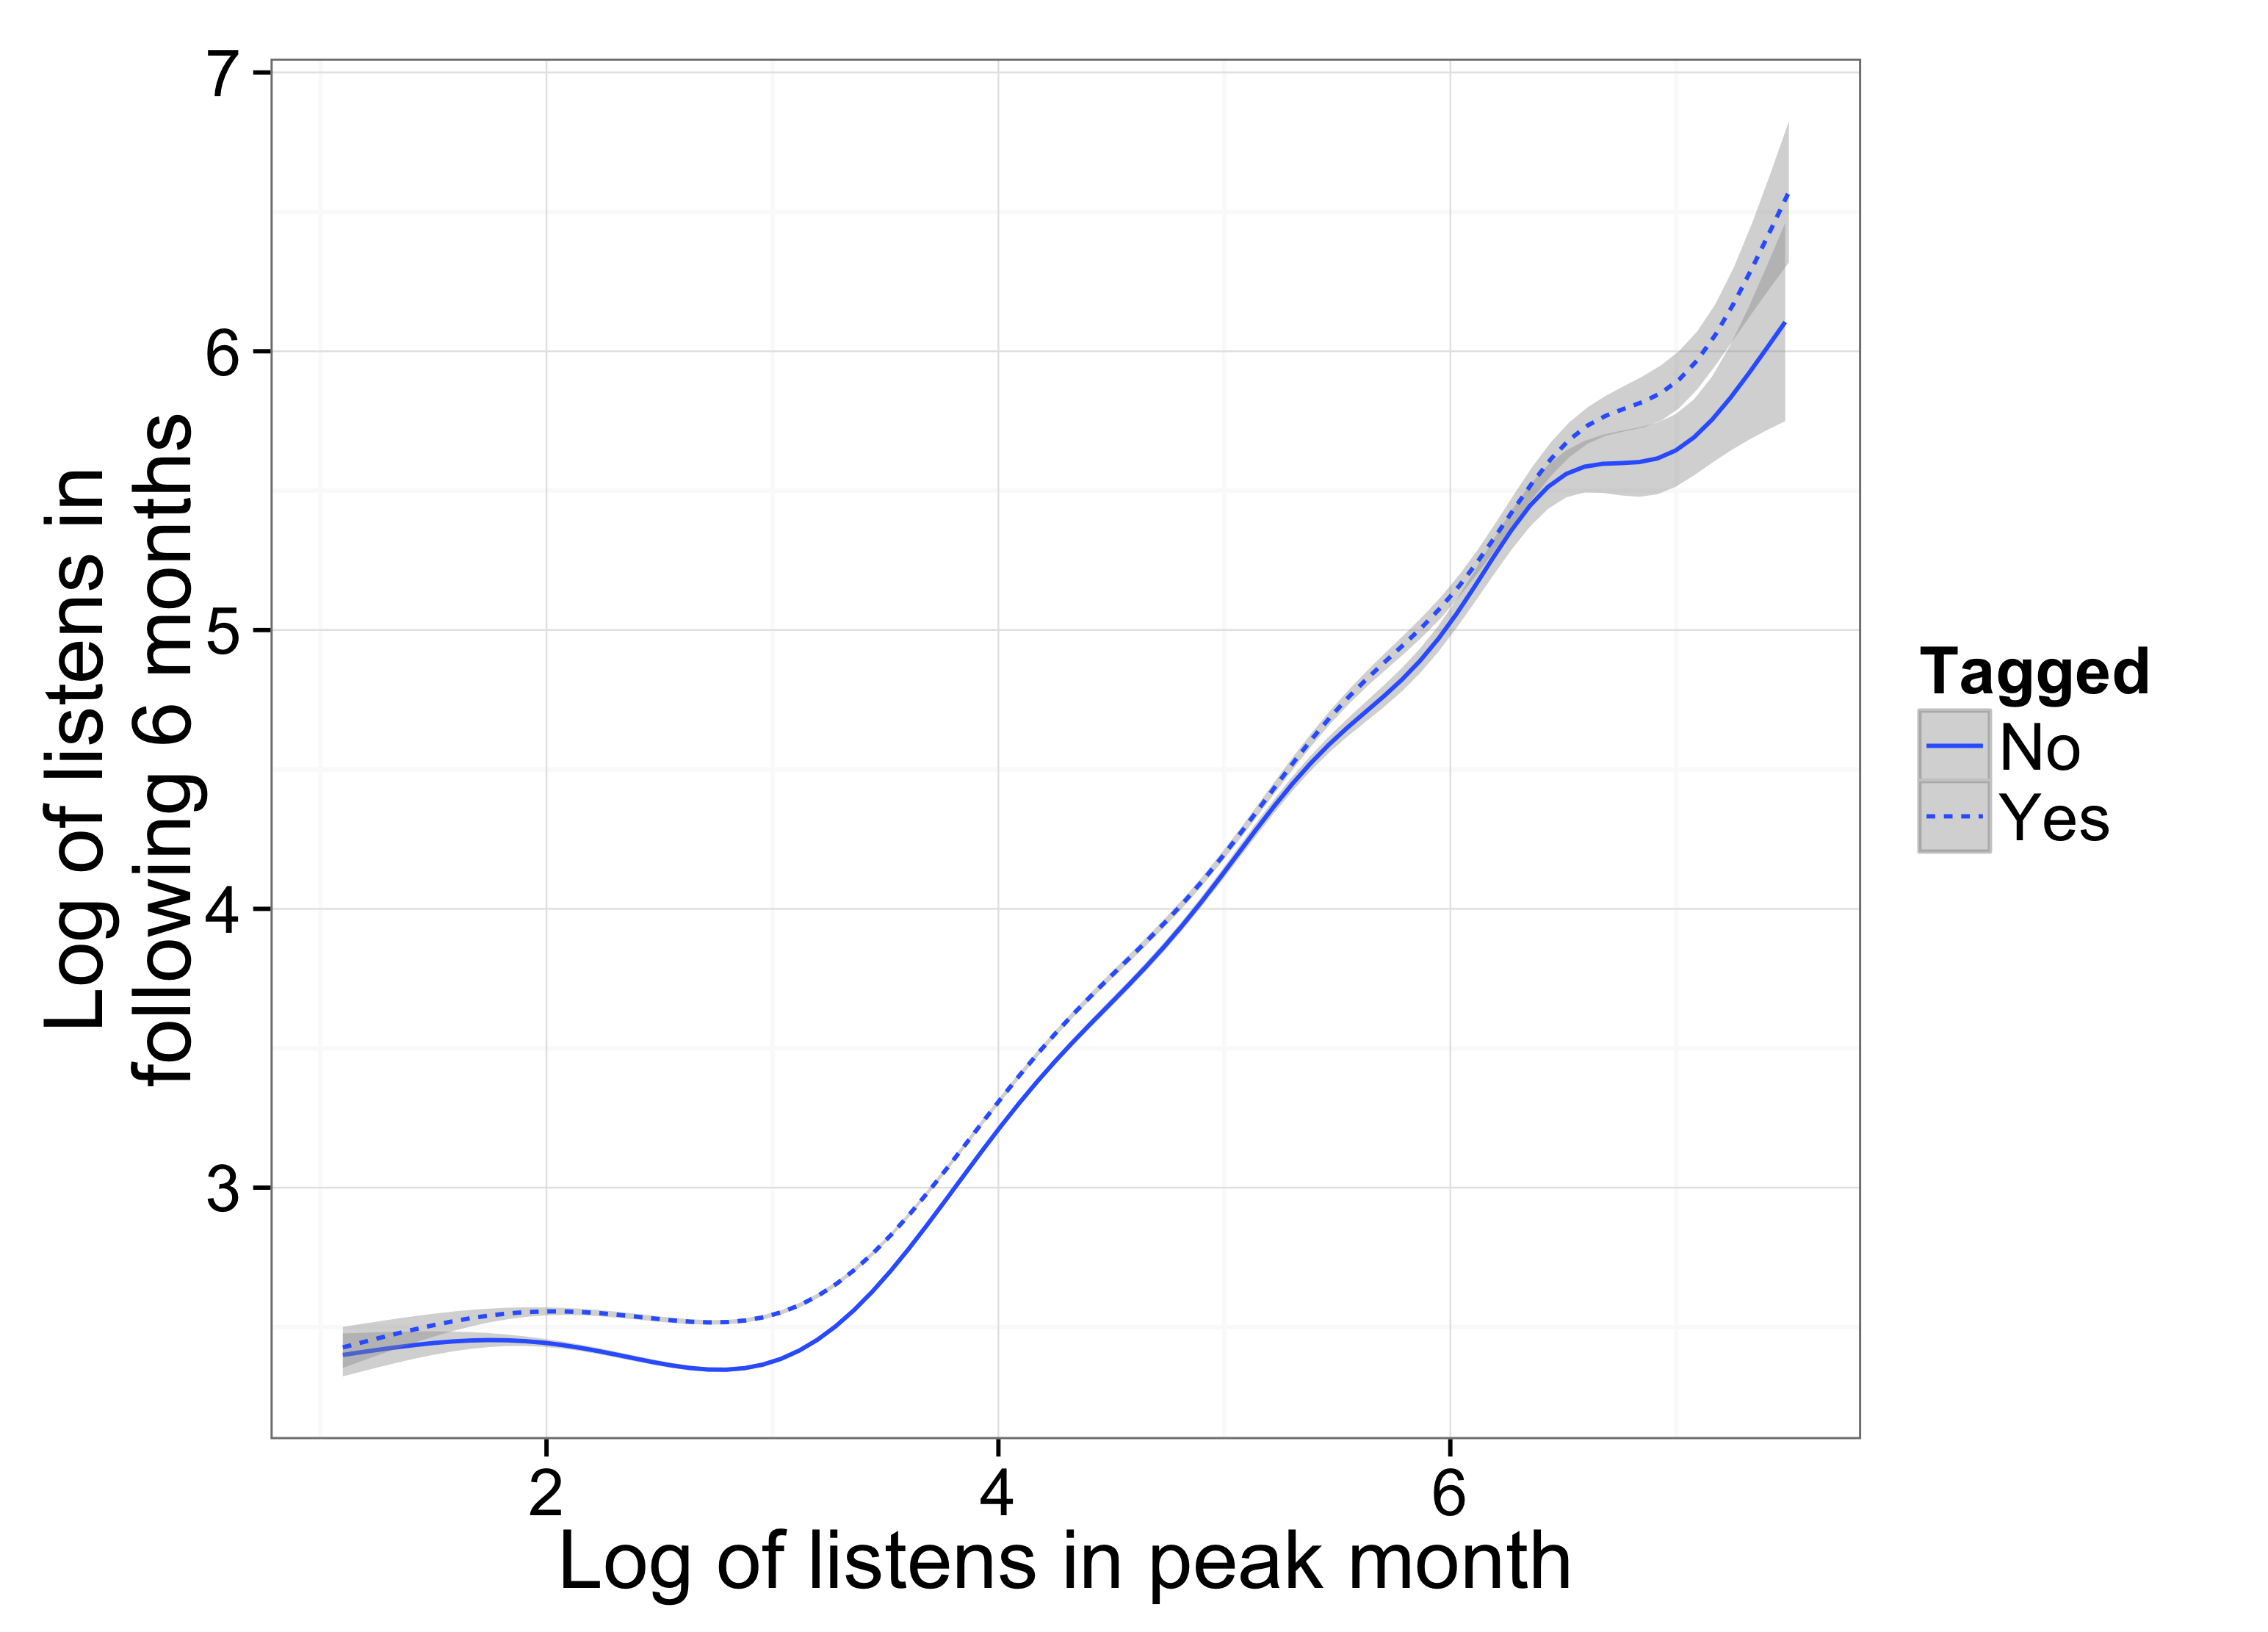
\includegraphics[width=0.45\textwidth]{taggedVUntaggedRegression.png}
    }
    \caption{Comparison of tagged and untagged listening time series}
    \label{fig:regressionFigs}
  \end{figure}

The regression model, which explained approximately 30\% of the variance in the data (adj. R-sq.), indicated that smoothed (using thin-plate regression splines) parameters for all seven previous months had a signficant effect on post-peak listening behavior. As we cannot show the form of this effect for all model variables, Figure~\ref{fig:regression} instead displays a similar model which considers only the effect of listening in the peak month on post-peak listening. As this plot suggests and the full model confirms, we can conclude that, controlling for all previous listening behavior, a tag increases the logarithm of post-peak listens by .147 [.144,.150]. This indicates that the effect of a tag is associated with around 1.15 more listens, on average, than if it were not to have been applied.   

\subsection{Tag analysis}
To examine if and how different tags are associated with increased future listening, we ran a regression analysis similar to that described above. Four important changes were made. First, as would be expected, we considered only tagged time series.  Second, instead of a single tagged/untagged indicator, we included binary (present / not present) regressors for all unique tags that had at least 25 occurrences in our subsample. Third, due to the data-hungry nature of the GAM and the large number of additional variables introduced by utilizing all tags as unique predictors, we chose to only control for listening in the peak month. This decision limited the computational difficulties associated with estimating a model of this size and did not appear to affect model fit substantially in subsamples of the data. Finally, we eliminated the constraint that a tag must occur in the peak month of a time series, as there is no meaninguful comparison to be made with untagged data in this analysis. This allowed us to include additional tagged time series. If users had multiple tags for a particular artist, we again selected one tag randomly rather than include the same user artist combination twice in our analyiss.

This expanded sample consisted of 600,701 tagged time series, with 6,060 unique tags. After running the model, which explains $\sim$16.7\% of the variance in the data (adj. R-sq.), 321 unique tags proved to be statistically significant predictors at $p <.001$. While we only have sufficient evidence to make claims about these 321 tags, qualitative examination of which tags are relatively strong predictors in the model proves informative.

The most telling observation is that commonly-used genre tags (e.g. ``pop'', ``jazz'', and ``hip-hop'') -- which are the most common tags overall in our full dataset -- tend to be weak, negative predictors of future listening. In contrast, relatively strong predictors (both positive and negative) appear to be comparatively obscure, possibly idiosyncratic tags (``arguman-loved tracks'', ``mymusic'', ``leapsandbounds cdcollection'').\footnote{For a full listing of the regression coefficients across all tags in the model, see \url{https://dl.dropboxusercontent.com/u/625604/papers/lorince.joseph.todd.2015.sbp.supplemental/regression_coefficients.txt}} To examine this trend quantitatively, we plot in Figure~\ref{fig:coefVsPopularity} global tag popularity (i.e. the total number of uses of a tag in our full dataset, which consists of $\sim 50$ million annotations) as a function of the tag's coefficient in the regression model for all tags that had a statistically significant coefficient. The red bands marked the upper and lower limits of a bootstrapped 95\% confidence interval on the popularity of the 5,739 remaining tags that were \emph{not} significant in the regression model. The result is a clear trend which suggests that the most popular tags are significant, weakly negative predictors of future listening, while both positive and negatively strong predictors tend to be relatively unpopular. Tags which were not significant in the model tend to be of moderate to high popularity.

  \begin{figure}[t]
	\centering
      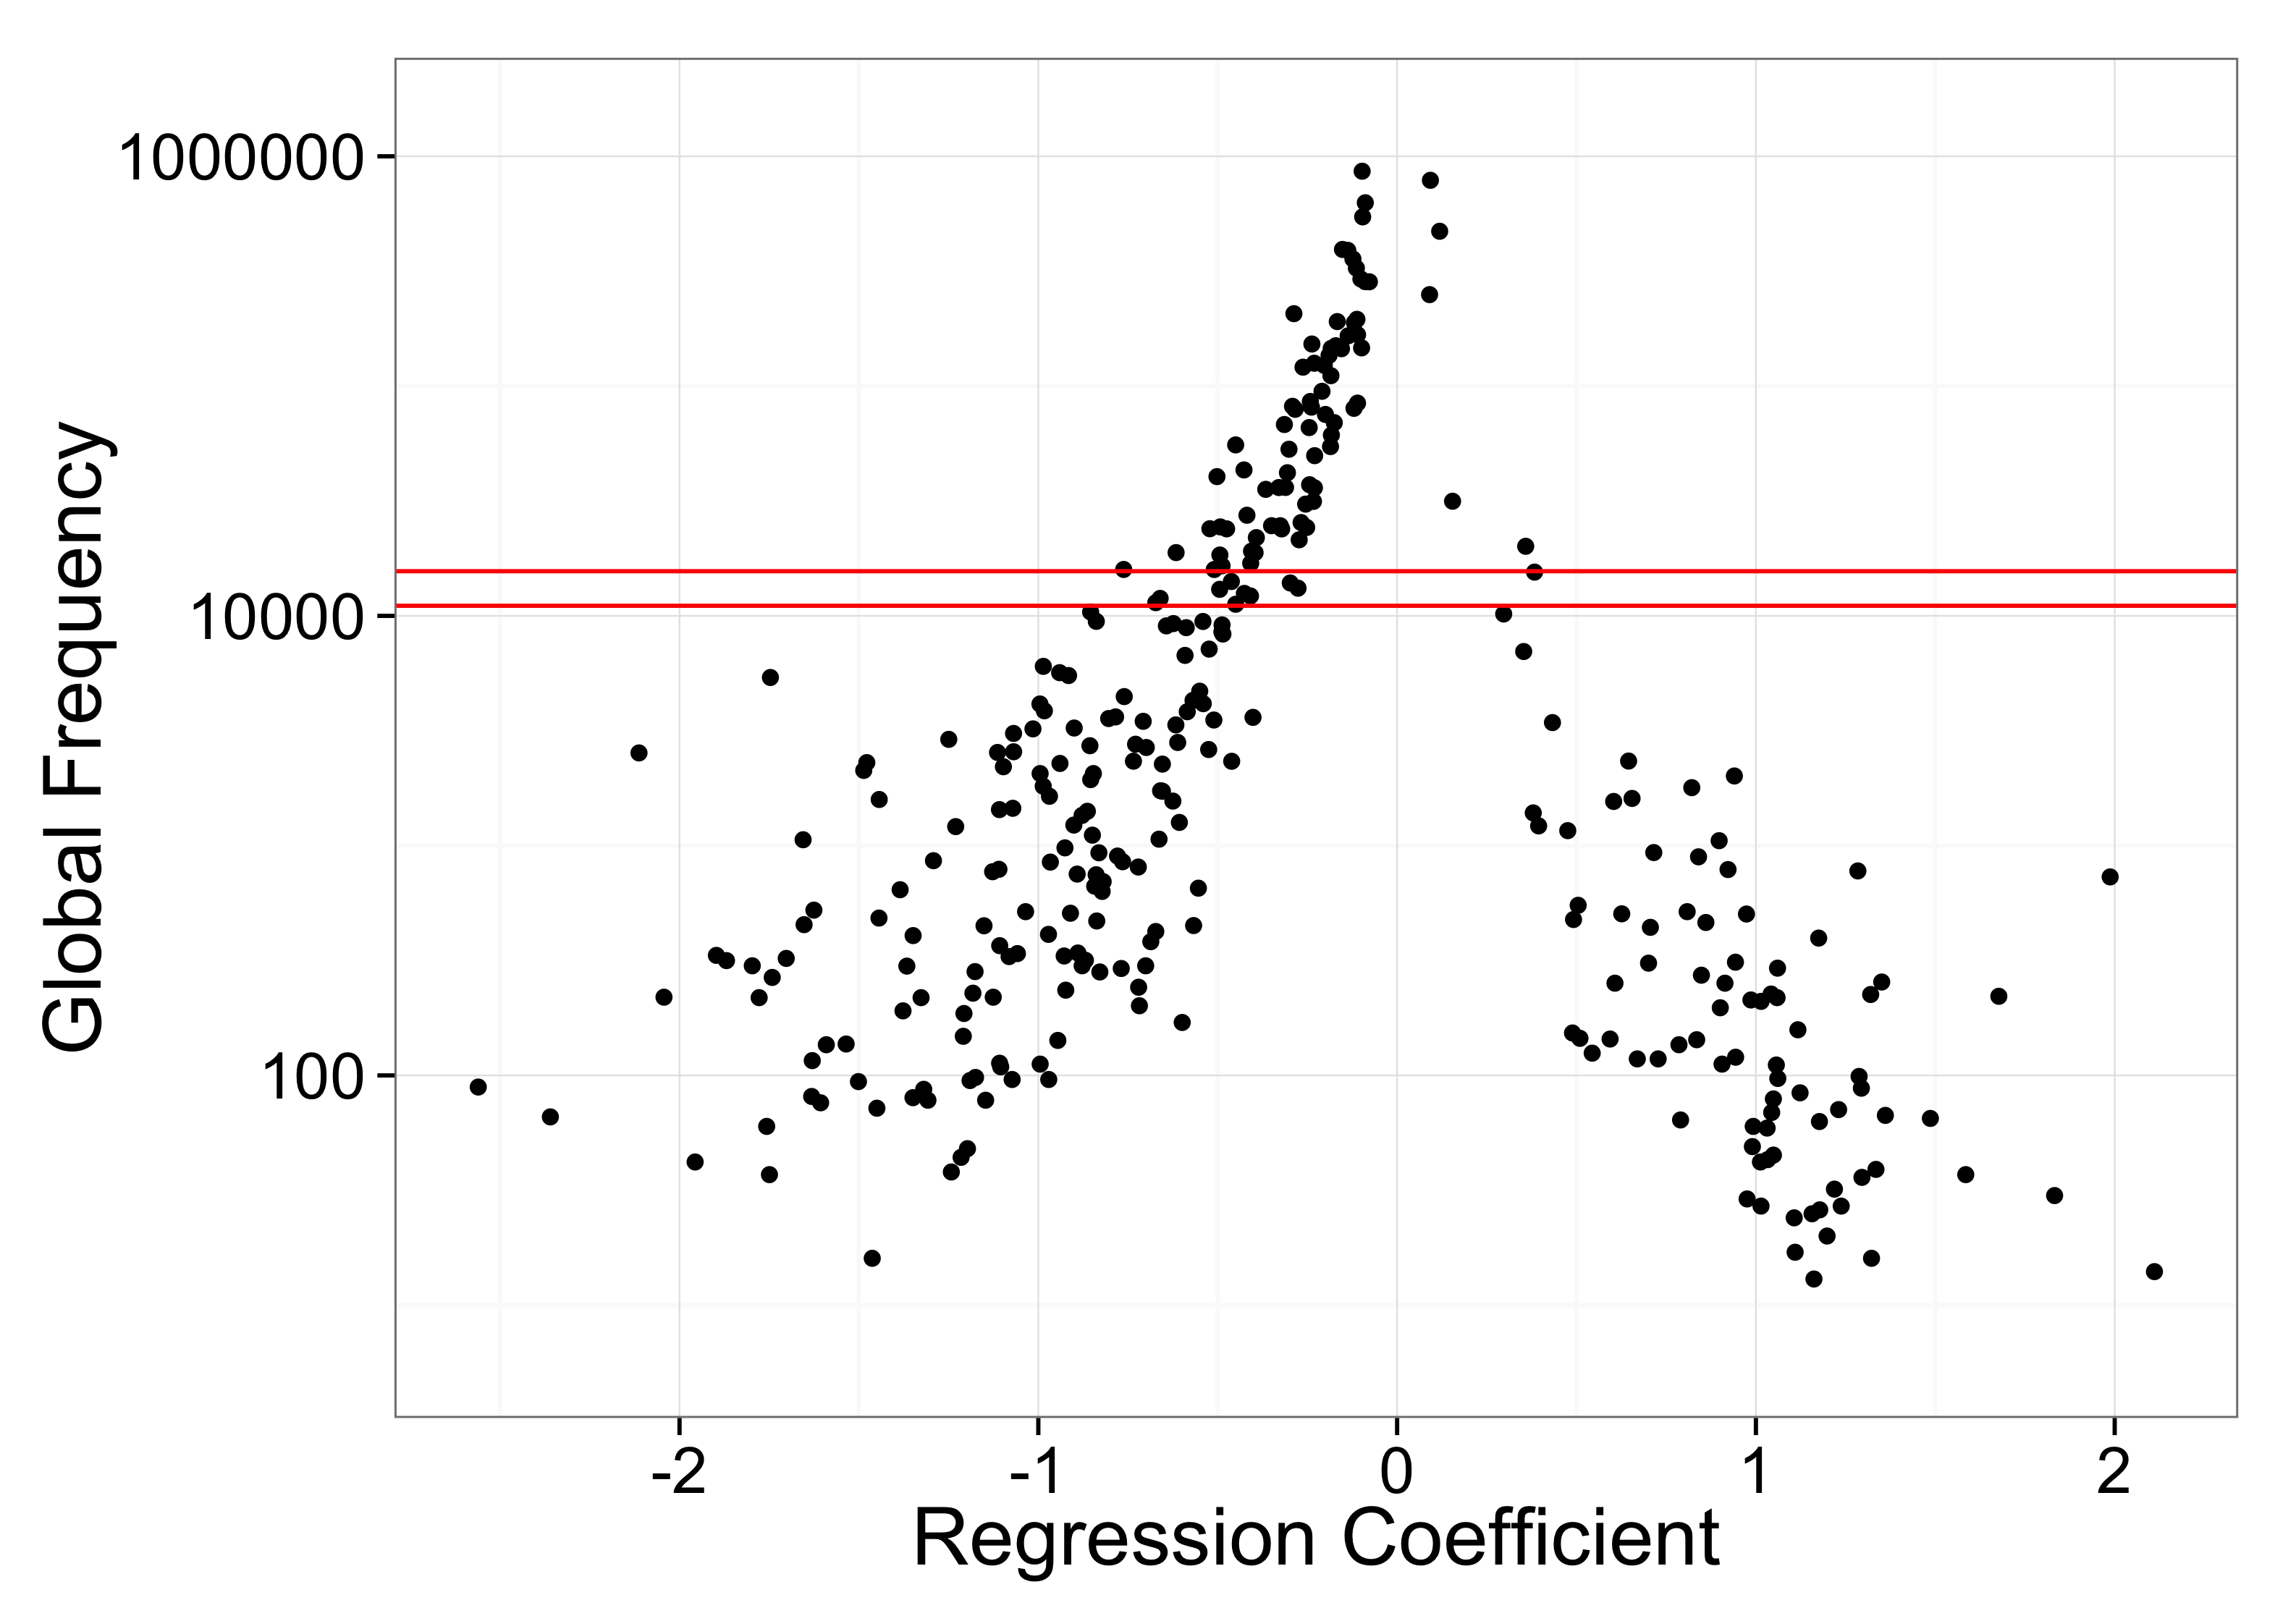
\includegraphics[width=0.7\textwidth]{tagRegressionWithMoreData.png}
    \caption{Logarithm of tags' global popularity as a function of regression coefficient.}
    \label{fig:coefVsPopularity}
  \end{figure}

These data suggest that, at least for the small number of tags about which we can make statistically meaningful claims, those that are globally popular and well-known have relatively little effect on future listening, and are generally associated with small \emph{decreases} in post-taggging listening rates. The tags that seem to ``matter'' (i.e. those that are relatively strong predictors of whether or not a user will listen to an artist after tagging it) are generally much less popular.